\documentclass{standalone}
\usepackage{tikz}
\begin{document}
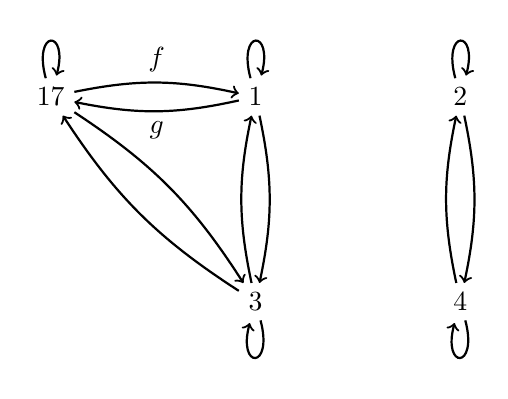
\begin{tikzpicture}[scale=1.3]
    \tikzset{arc lines/.style={thick,black, ->, bend left=12}}
    % \draw (0, 0) grid (6, 2);
    \node (17) at (0, 2) {$17$};
    \node (1) at (2, 2) {$1$};
    \node (2) at (4, 2) {$2$};
    \node (3) at (2, 0) {$3$};
    \node (4) at (4, 0) {$4$};
    \draw [arc lines] (17) to node[above] {$f$} (1);
    \draw [arc lines] (1) to node[below] {$g$} (17);
    \draw [arc lines] (17) to (3);
    \draw [arc lines] (3) to (17);
    \draw [arc lines] (1) to (3);
    \draw [arc lines] (3) to (1);
    \draw [arc lines] (2) to (4);
    \draw [arc lines] (4) to (2);
    \path [-stealth, thick]
        (1) edge [loop above] (1)
        (17) edge [loop above] (17)
        (2) edge [loop above] (2)
        (3) edge [loop below] (3)
        (4) edge [loop below] (4)
        ;
\end{tikzpicture}
\end{document}
